\chapter{Using the workspace}\label{ch:workspace}
\chapterlead{The workspace is where you inspect structures, organize calculations, and retain results. This chapter introduces the main window, then takes you through importing, inspecting, naming, and saving a silicon project. These habits will carry through the later tutorials.}

\section{The main window}
\index{Workspace}
The workspace brings structures, calculation steps, and results into one window. Start by recognizing the empty layout, then open the panels needed for an exercise. This helps distinguish what the project contains from what you are editing at the moment. The ribbon selects commands, the central document area displays structures, workflows, and figures, and the side panels hold project items, object information, parameters, and output.

\subsection{Your first view of the workspace}
An empty project initially shows a welcome message with no structure or workflow document open. Figure~\ref{fig:desktop-start} shows this layout: the Project Browser lists categories on the left, the Information Browser below it is collapsed to its title bar, and the right-side panel group is closed. Import a structure or create a workflow to open its document in the central area.

\begin{figure}[!htb]
\centering
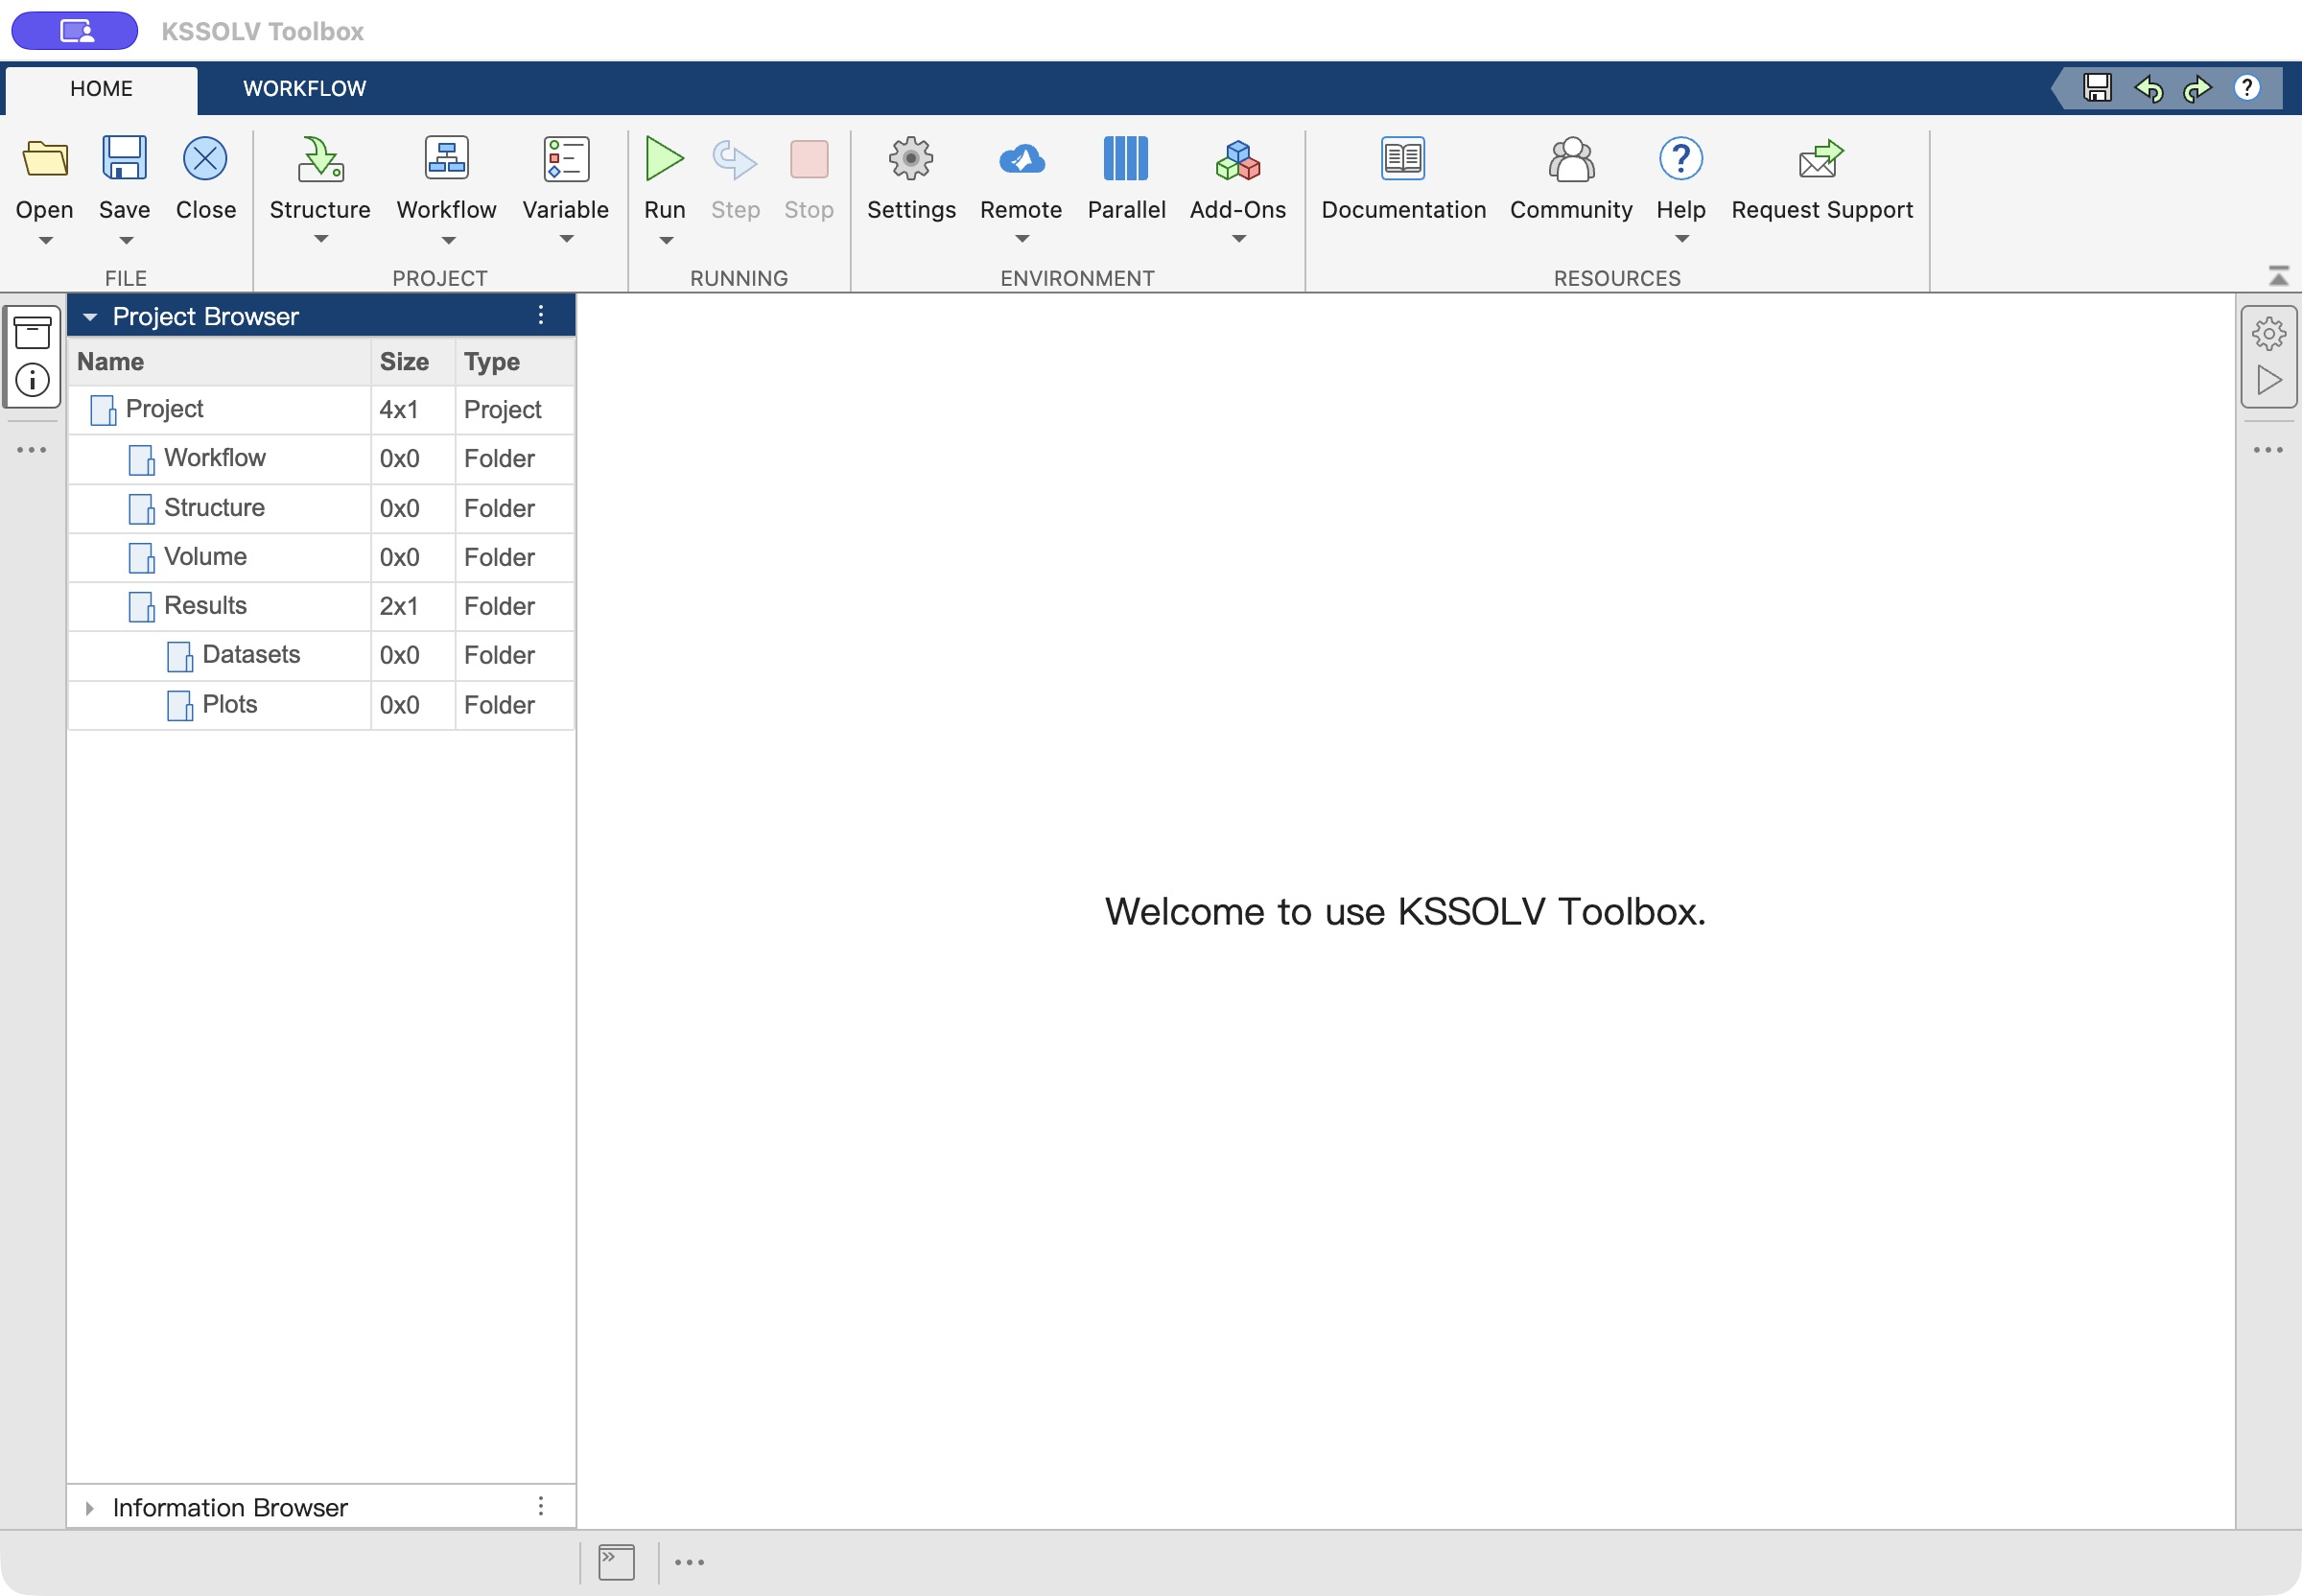
\includegraphics[width=\linewidth]{publication-assets/crop-eb25a0cdb09d3f78fdbd.png}
\caption{The initial desktop workspace. No document is open in the center. The Project Browser lists project categories; the Information Browser is collapsed to its title bar, and the right-side panel group is closed.}
\label{fig:desktop-start}
\end{figure}

Locate \ui{Structure} and \ui{Workflow} on the \ui{Home} tab, then inspect the buttons at the sides. Project and information buttons control one panel group on the left; configuration and simulation buttons control another on the right. A group button collapses or expands that side's region. The small triangle in an individual panel title expands its contents. If a panel is missing, open the sidebar ellipsis and select it by name from \ui{Open Panels}.

\subsection{Open the panels needed for an exercise}
Your first calculation involves moving between the project, structure, workflow, and parameters. Figure~\ref{fig:install-workspace-overview} shows an empty project with the main panels expanded: project and information on the left, configuration and simulation on the right, the Command Window below, and the welcome message in the center. Some panels are collapsed on first launch.

Expand the two side groups and their individual panels to learn their locations. Importing a structure or creating a workflow adds items to the tree and document tabs in the center. Double-click a project item to open its document, then select a tab to make it active. A structure tab shows a 3D model; a workflow tab shows nodes and connections. Check the active workflow's name before configuring nodes or running a calculation.

\begin{table}[!htb]
\centering
\caption{Main workspace areas and what to look for first.}
\label{tab:workspace-regions}
\begin{tabularx}{\linewidth}{p{24mm}p{32mm}X}
\toprule
Area & Location & First check \\
\midrule
Ribbon & Top of the window & Find structure import, workflow, save, and run actions on \ui{Home}. \\
Quick Access Toolbar & Upper-right corner & Identify Save, Undo, Redo, and Help. \\
Project and information & Left-side group & Recognize the categories, then select an imported structure to view its information. \\
Configuration and simulation & Right-side group & Locate parameters and output. After creating a workflow, select a node to configure it. \\
Document area & Center & An empty project shows the welcome message. Use tabs to switch between open structures and workflows. \\
Command Window & Expanded lower region & Use it for interactive commands when needed; it can stay open or collapsed during graphical tutorials. \\
Dividers and status bar & Panel boundaries and window bottom & Drag dividers to adjust space and watch the status text during operations. \\
\bottomrule
\end{tabularx}
\end{table}

Adjust the layout to suit the task. Collapse unused side panels to inspect a 3D structure, or widen the Config Editor when entering parameters. Drag panel boundaries to change widths or vertical proportions; structures and workflows remain in the project. The following sections explain the areas in detail, and the silicon exercise puts them to use.

\subsection{The ribbon}
\ui{Home} groups common file, project, run, environment, and resource actions. \ui{Open} reads an existing project, and \ui{Save} writes the current work to a project file. \ui{Structure} creates or imports structures; \ui{Workflow} provides creation, template, import, and export actions. Use \ui{Run} to execute a calculation. Settings and help are also available from Home.

The \ui{Workflow} tab provides node and canvas operations for the central workflow document. Activate the intended workflow before adding, connecting, or configuring nodes. Selecting the ribbon tab alone does not identify which workflow will run; check the central document tab too.

When a 3D structure document is active, \ui{Crystal Modeling} or \ui{Molecule Modeling} appears on the ribbon. These contextual tabs provide tools for the current document and may change when you switch document types. If a modeling command is missing, return to the structure tab before considering another import.

\subsection{Project Browser}
\index{Project Browser}
The Project Browser presents project contents as a tree. Its main branches are \ui{Workflow}, \ui{Structure}, \ui{Volume}, and \ui{Results}. Results contains \ui{Datasets} and \ui{Plots}. These correspond to workflows, atomic structures, volumetric data, numerical data, and figures.

Single-click an item to select it, or double-click to open its document. A project can retain many items at once. Closing a central document tab closes that view; it does not delete the item. Double-click the item again to reopen it. A removal action, by contrast, changes the project contents.

\ui{Name} is the display name, \ui{Type} identifies the object type, and \ui{Size} describes item organization or data dimensions. Do not interpret Size directly as the atom count. Read structure information or the site count in the 3D view to find the independent atoms in a crystal. Displayed spheres may include neighboring-cell images and need not equal the model's site count.

\subsection{Information Browser}
The Information Browser follows the Project Browser selection. Select a structure to inspect its properties, or a workflow, dataset, or figure to inspect that object. Use it to confirm which item you are working with, especially when names are similar.

Some items allow their display names to be edited. Check the updated name in both the tree and document tab. Names describing the material and principal change, such as \file{Si-primitive}, \file{Si-2x2x2}, or \file{Si-vacancy}, are more informative than \file{Structure1}. Cell details and atom counts remain available in the structure information.

\subsection{Config Editor}
\index{Config Editor}
The Config Editor changes workflow-node parameters. Select a node on the canvas, then choose \ui{Workflow → Configure Node} or use the node's gear button. Scroll down to its \ui{Options}. General fields such as the node name, inputs, and outputs are separate from task parameters such as cutoff energy and iteration limits. If only general fields are visible, invoke Configure Node before scrolling. After entering values, switch to another node and back to check that the entries were committed.

\subsection{Read run output}

The \ui{Simulation Browser} displays calculation output, including SCF iterations, messages, and errors. After a run, inspect its final messages and the new items under Results. Chapter~\ref{ch:first} demonstrates how to judge completion using a small calculation.

\subsection{Arrange the panels}
\index{Sidebars}
The document area can hold structure, workflow, and figure tabs simultaneously. Selecting a tab changes the active document. If tabs are hidden, move the pointer to the top of the document area to reveal document titles and tabs. Check the active workflow name before running. Clear names help avoid running the wrong one when several similar tasks are open.

The sidebars control panel groups. Project and information icons belong to the left group; configuration and simulation icons belong to the right. Collapsing the left group hides both the Project Browser and Information Browser; expanding it makes both available again. The right group similarly allows configuration and output to be viewed together. Figure~\ref{fig:desktop-start} shows the right group collapsed, while Figure~\ref{fig:install-workspace-overview} shows the manually expanded layout.

Individual panels can also be collapsed. The initial \ui{Information Browser} shows only a title bar at the lower left; click its triangle to reveal the contents. Collapsing a panel affects just that panel, whereas collapsing the side group hides the entire region.

The sidebar ellipsis opens \ui{Open Panels}. Select \ui{Project Browser}, \ui{Information Browser}, \ui{Config Editor}, \ui{Simulation Browser}, or \ui{Command Window} by name if you cannot find it. Figure~\ref{fig:panels-gallery} shows the Online list, which also includes \ui{Files} for server-side storage. The other five panels are available in the standalone application too.

\begin{figure}[!htb]
\centering
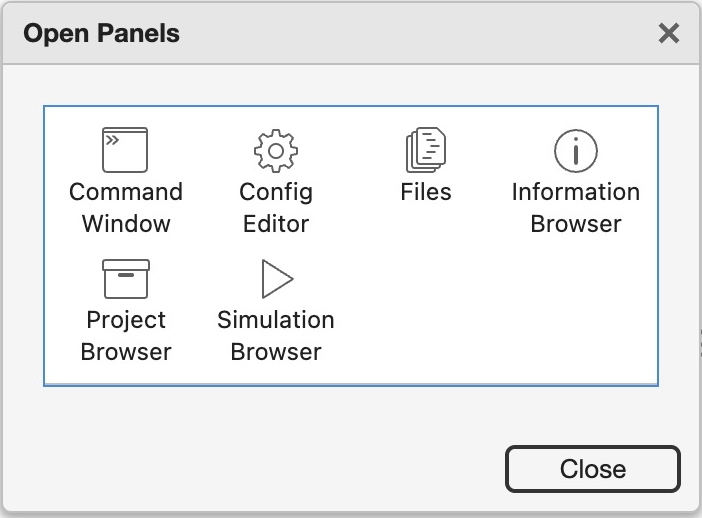
\includegraphics[width=88mm]{publication-assets/crop-50f2208998010f44014c.png}
\caption{The panel list. Open an individual panel by name; sidebar buttons collapse or expand panel groups. Files manages server-side storage.}
\label{fig:panels-gallery}
\end{figure}

Collapse unused parameter and output panels while inspecting a model, then reopen configuration when needed. Drag the dividers between panels and documents to change widths, or the divider within a group to change vertical proportions. Choose widths appropriate to your screen.

\section{Exercise: import and inspect silicon}
The supplied \file{silicon.cif} describes a conventional silicon cell with sides of approximately $5.44370\,\text{\AA}$ and 8 explicitly listed sites. It uses P1 to list every position, making the atom count easy to check. The lattice constant is an input to this example, not a result calculated during import.

\begin{figure}[!htb]
\centering
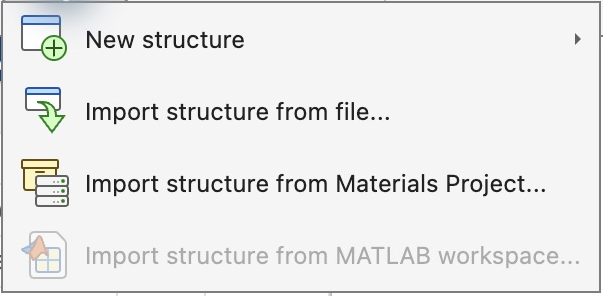
\includegraphics[width=67mm]{publication-assets/crop-e572efea8aa253089edc.png}
\caption{The Structure menu on Home. This exercise uses \ui{Import structure from file...}. Materials Project is another source. Importing from the MATLAB\regmark{} workspace requires the MATLAB\regmark{} toolbox edition.}
\label{fig:structure-import-menu}
\end{figure}

\begin{steps}
\item Open \ui{Structure} on \ui{Home}, then choose \ui{Import structure from file...}.
\item Select \file{silicon.cif} in the supplied example directory and open it.
\item Wait for \file{silicon} to appear under \ui{Structure} and for its 3D document to open.
\item Drag to rotate and use the mouse wheel to zoom. Fit the whole cell in the view; there is no need to adjust every display setting immediately.
\item Check that the element is Si and there are 8 independent sites. Any extra spheres may be boundary or neighboring-cell images.
\item Select a site to inspect its atom information, then clear the selection using empty space or the appropriate selection action to view the complete structure again.
\end{steps}

\begin{figure}[!htb]
\centering
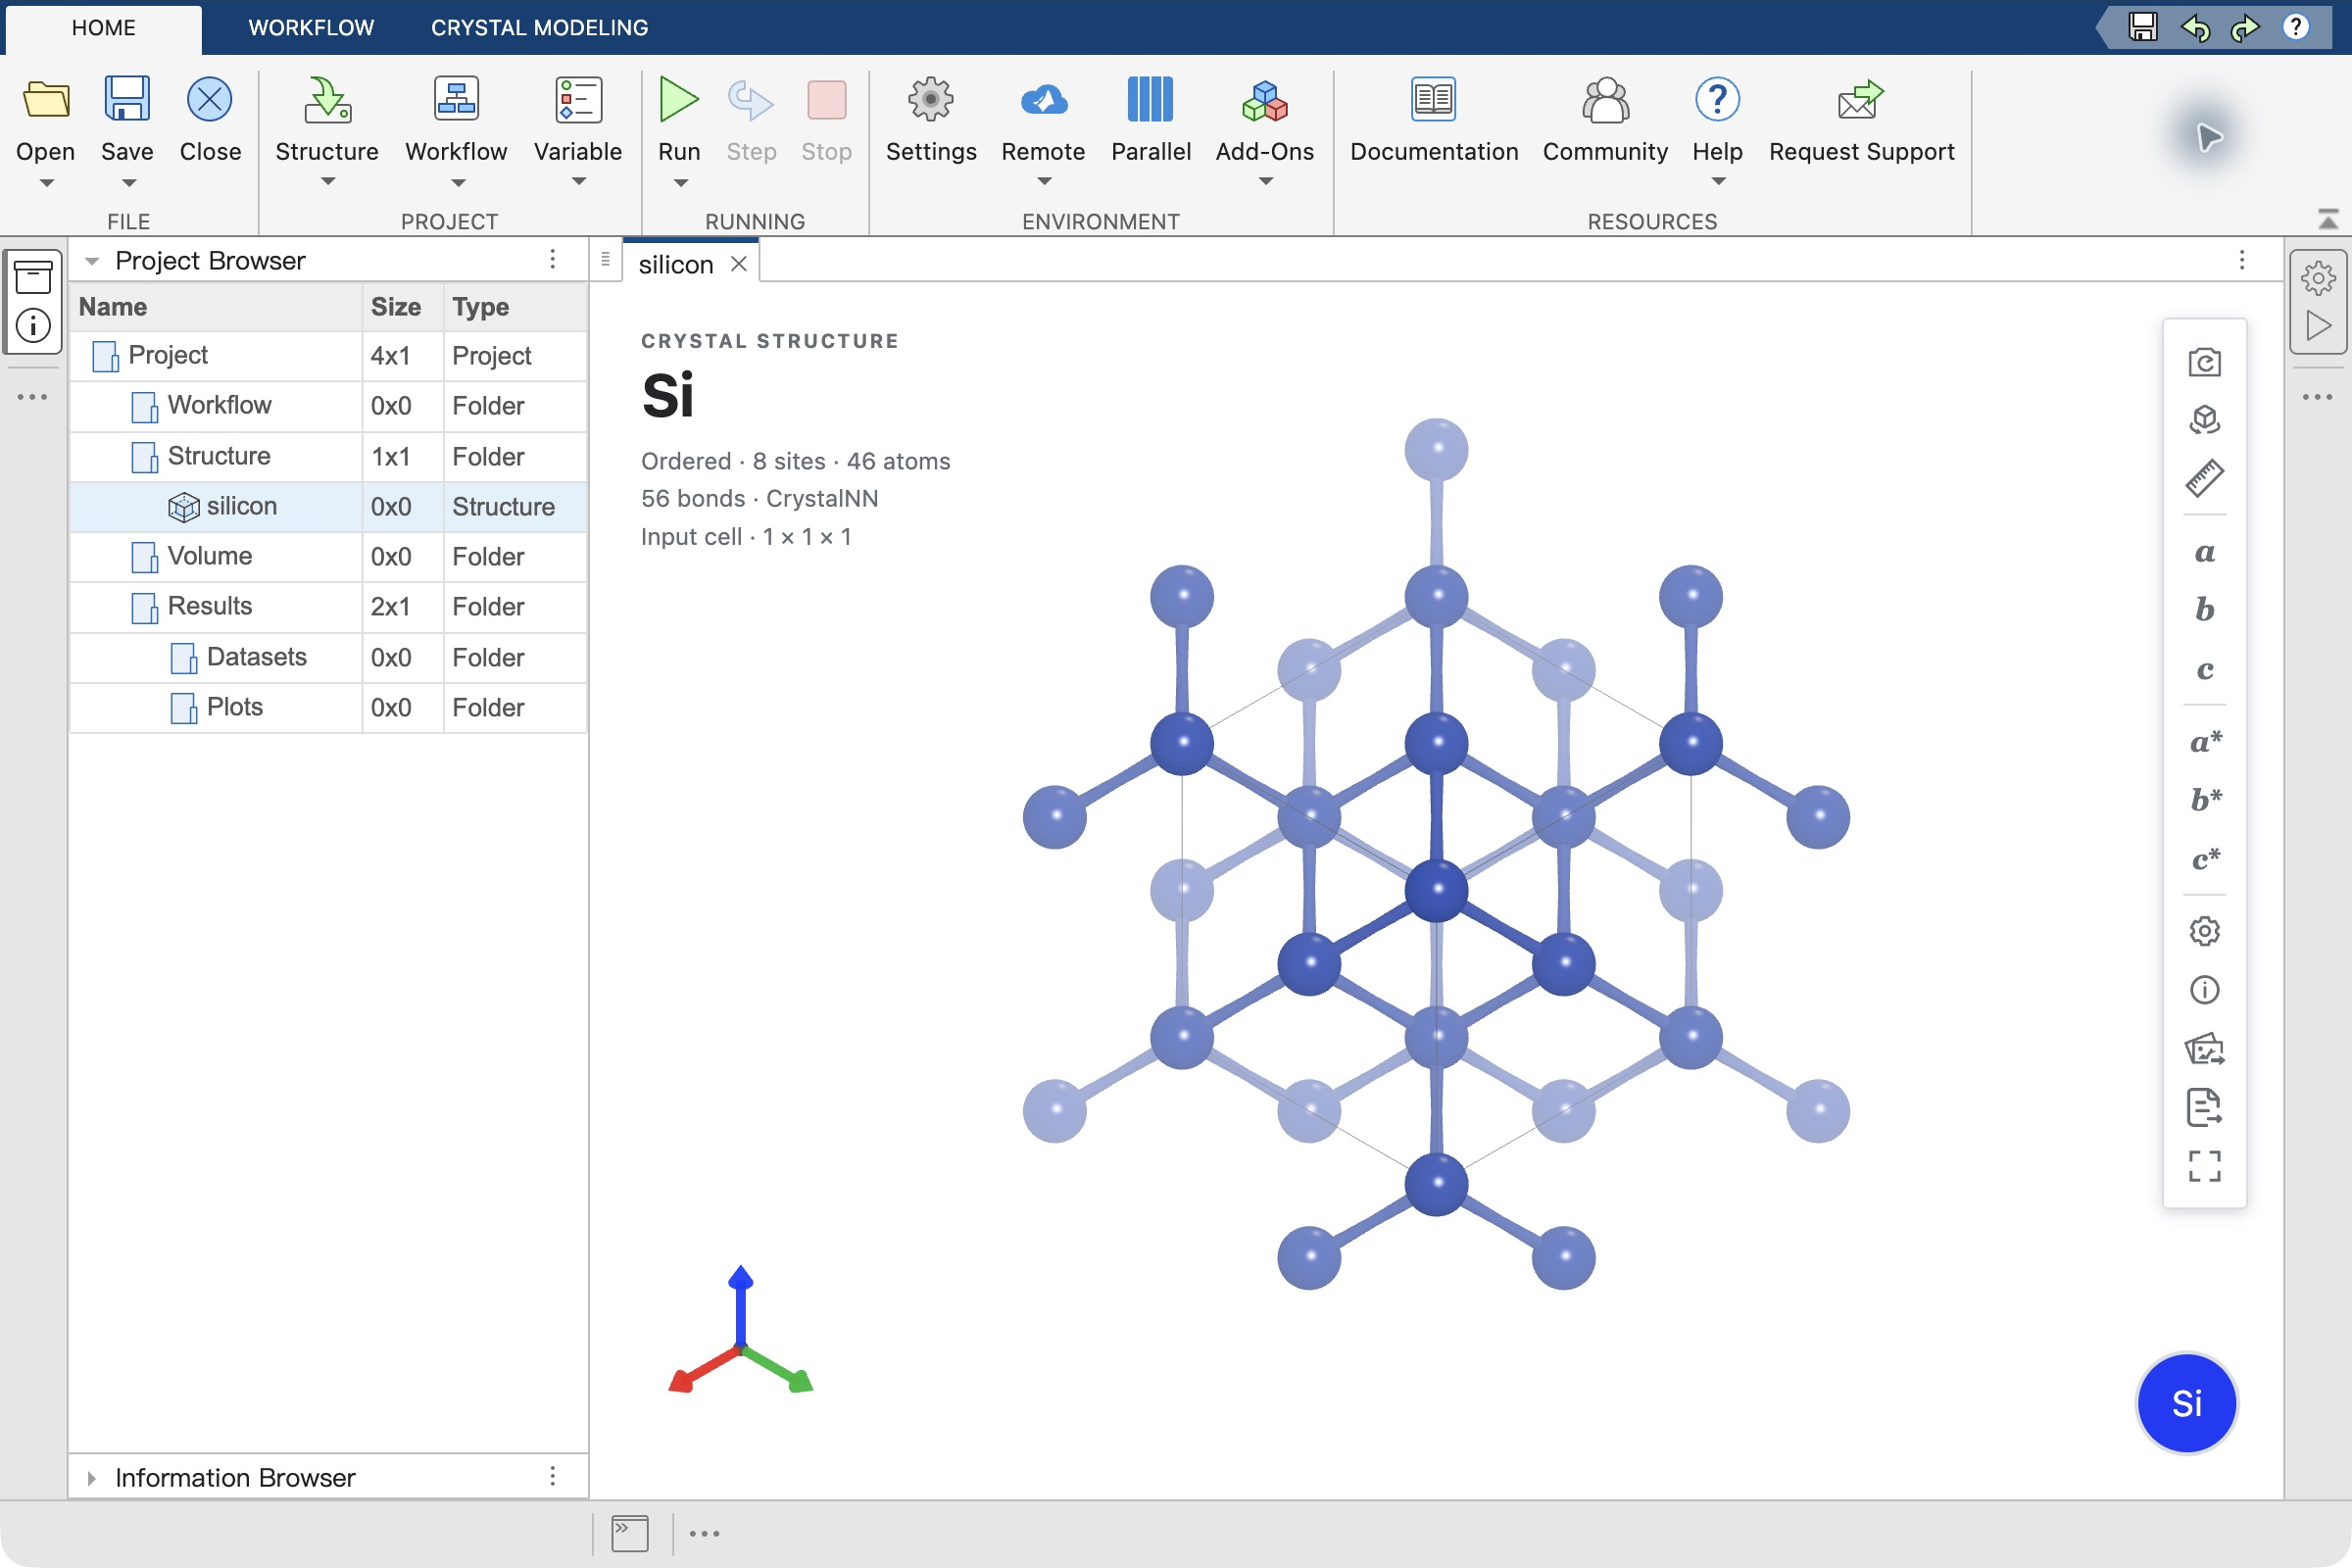
\includegraphics[width=\linewidth]{publication-assets/crop-693a9be4f512a9a0e125.png}
\caption{The imported silicon structure. The summary reads \ui{8 sites · 46 atoms}: 8 independent input sites and 46 displayed spheres including periodic boundary images.}
\label{fig:silicon-import}
\end{figure}

\subsection{Import several files at once}

The desktop file picker allows multiple structure files to be selected. Use \ui{Import structure from file...} and open the selected inputs together when comparing models. Each successfully read file becomes a separate project structure; the atoms are not automatically combined into one model.

Open each added item under Structure to inspect it. If an individual file fails to parse, address its diagnostic separately; the other imported structures remain in the project. In Online, upload the files first, then import them individually through Files. A successful upload does not itself import a structure.

\subsection{Read site information}
The upper-left summary describes the structure and current display. Here, \ui{8 sites} refers to the eight silicon positions in the file; \ui{46 atoms} includes the periodic images drawn near the boundaries. \ui{Input cell · 1 × 1 × 1} indicates the input-cell display. Additional boundary spheres clarify connections across cells without turning the model into 46 independent atoms.

Select a silicon--silicon bond to inspect its sites and geometric length. Figure~\ref{fig:silicon-bond-inspection} shows \ui{Sites 2–7}, a length of $2.35719\,\text{\AA}$, and image indices \ui{0, 0, 0}. Site indices identify atoms in the model; image indices identify the cell translation used by that connection. Check both when inspecting other bonds.

\begin{figure}[!htb]
\centering
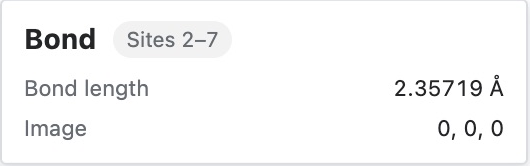
\includegraphics[width=79mm]{publication-assets/crop-6bd0b3f7b04c691f91a8.png}
\caption{The inspection card for a selected silicon--silicon bond. Its length of $2.35719\,\text{\AA}$ is a geometric property of the input structure.}
\label{fig:silicon-bond-inspection}
\end{figure}

Clear the selection afterward to restore the complete view. The aim is to understand how file contents, model sites, and displayed images relate. Use the same checks after building a supercell or optimizing a structure: read the structure information first, then inspect relevant atoms and connections.

For a CIF from another source, check the cell, occupancies, elements, and atom count after import. Files may use primitive cells, conventional cells, or partial occupancies. An identical chemical formula does not guarantee an identical structure. Understand the file's representation before converting or expanding it.

\section{Save the project}
\index{Saving projects}
\subsection{The first save}
\begin{steps}
\item Click \ui{Save} on \ui{Home}.
\item In the standalone edition, choose your working directory and enter \file{Si-introduction.ks}. In Online, choose a server-side directory as described in Chapter~\ref{ch:online}.
\item After saving, check the window title and project filename.
\item Make a small, recognizable change, such as renaming the structure, and observe the asterisk in the title.
\item Save again and confirm completion.
\end{steps}

An asterisk indicates unsaved changes. Saving retains workflows and results as well as pending structure edits. Modeling has distinct preview, apply, and save stages: preview checks a proposed change, Apply accepts it, and Save writes the current work into the project file. Chapter~\ref{ch:modeling} demonstrates them through editing exercises.

\subsection{Keep copies for different studies}
Use \ui{Save As...} to branch a project for different conditions. For example, save the original silicon project, then save a copy as \file{Si-supercell.ks} before building a supercell. This retains a clear starting point. Renaming a project does not change the model; inspect the structure to confirm that the intended operation was performed.

For cutoff comparisons, you can keep several clearly named workflows in one project. Separate projects may be easier to organize if results are numerous or substantially different. Either approach is valid as long as results can be traced to their structures and parameters.

\subsection{Reopen and check}
Close the project and use \ui{Open} to read the saved \file{.ks} file. Expand Structure, double-click silicon, and check that its view reopens. This confirms that you saved a usable project rather than merely an image of the screen.

In Online, opening a saved server-side project and opening a downloaded local copy use different routes. Select the existing \file{.ks} in Files for the former; upload the local copy first for the latter. The contents may be identical, but check the storage location.

\subsection{Close the current project}

\ui{Home → Close} closes the entire current project, not just one central structure tab. Unsaved project or structure changes trigger a prompt to save, discard, or cancel. Choose \ui{Cancel} to stay in the project. If saving, wait for completion before the empty project opens. Closing a document tab instead retains its tree item for reopening.

\subsection{Remove trial items}

Remove workflows, structures, or figures you no longer need from the project. Save a separate project copy first if you want to retain a milestone.

\begin{steps}
\item Select the specific trial item in the Project Browser, rather than Project or a category folder.
\item Keep focus in the tree and press Backspace to remove it. A workflow can also be removed by selecting its project item and choosing \ui{Delete} on the Workflow tab.
\item If its document has unsaved changes, respond to the close prompt. If you cancel, return to the tree and check the selection.
\item Check that the remaining structures and workflows still correspond, then save. Removing a project item does not delete its original source file from disk.
\end{steps}

\section{Choose what kind of file to save}
\index{Project files}
\file{.ks} stores the complete project; \file{.wf} stores a workflow; CIF, POSCAR, and XYZ mainly store structures. Choose according to what a collaborator needs. A project is usually best for continuing a calculation. A workflow template is useful for reusing task organization with another material. Export a structure file when only geometry is needed.

Each structure format retains different information. CIF is suited to cells and crystal positions. XYZ directly represents elements and Cartesian coordinates, but ordinary XYZ does not fully specify periodic cells or explicit bonds. When saving important molecular connectivity or a complex periodic model, check what the chosen format supports and inspect the result after reimporting it.

\section{Use the Command Window}
\index{Command Window}
The Command Window is an additional entry point for interactive commands. Standalone and Online sessions support the functions and built-in operations included in their distribution. The supplied reproducibility scripts run in full MATLAB\regmark{}. Normal import, modeling, and workflow tutorials do not require this window. Before using a command, check that it addresses the intended workspace object, then verify the result in the tree or view.

\ui{Documentation} and \ui{Help} on Home provide further reading; \ui{Help → About KSSOLV} shows version information. If behavior differs from this manual, first check the version and active document type. Chapter~\ref{ch:troubleshooting} explains how to prepare a problem report and collect logs.

\subsection{Run a simple command}

Open \ui{Command Window} from \ui{Open Panels} and place the cursor in the input area after \texttt{>>}. Press Enter to submit a command; its output appears below. This exercise uses a simple array without changing project structures.

\Needspace{5\baselineskip}
\begin{lstlisting}[language=Matlab]
a = [1 2 3];
sum(a)
\end{lstlisting}

Submit the lines separately; the second should return 6. Use \texttt{whos} to inspect variables in the command workspace. Up and Down recall previous commands, Tab selects completion suggestions, and Esc closes suggestions. \texttt{clc} clears the displayed history without deleting variables. Copy any commands and output you need into your notes before clearing it.

Command variables and project items are stored differently. Creating \texttt{a} does not add a structure to the project, and saving a project does not save every temporary command variable. Check the corresponding tree items when retaining structures, workflows, and results. For repeatable command sequences, prepare a script in full MATLAB\regmark{}.

\section{Use the Quick Access Toolbar}

The toolbar at the top provides Save, Undo, Redo, and Help. Quick Save saves the same project as \ui{Home → Save}; it does not export the current figure. With several documents open, check which is active: Undo and Redo address structure-modeling history in a structure document and graph-editing history in a workflow document.

\begin{steps}
\item Make a recognizable edit in the 3D structure and observe the change.
\item Click \ui{Undo} to return to the previous state, then \ui{Redo} to restore the edit.
\item Once the model is correct, click \ui{Save} and check the save indicator.
\end{steps}

After creating the first workflow in Chapter~\ref{ch:first}, move a canvas node and try Undo and Redo to compare these two editing contexts.

Saving files, running calculations, and undoing edits are separate operations. Undo does not restore external files or reverse a completed scientific calculation. Retain separate results and explicit parameter records when comparing calculations.

\section{Find structures in \headinglatin{Materials Project}}\label{sec:mp-search}
\index{Materials Project!Structure search}

A database search provides a starting structure when you do not yet have a local file. Save your Materials Project API key in Settings as described in Chapter~\ref{ch:remote}, then choose \ui{Home → Structure → Import structure from Materials Project...}. Query conditions appear at the top, the periodic table in the middle, and results with pagination below. After import, create a calculation workflow for the selected structure.

\subsection{Choose a search mode}

\begin{table}[htbp]
\centering
\caption{The three Materials Project search modes.}
\begin{tabularx}{\linewidth}{lX}
\toprule
Mode & Use \\
\midrule
Only these elements & Results contain every selected element and no others. Select only Si to search elemental silicon. \\
At least these elements & Results contain the selected elements and may include others. Select Fe and O, for example, to search materials containing both. \\
Formula / MP ID & Enter a formula or known material identifier to locate a particular record. \\
\bottomrule
\end{tabularx}
\end{table}

The first two modes use periodic-table selections, with the element text updating above. Switch to \ui{Formula / MP ID} for a formula search. \ui{Clear elements} removes the current selection before you choose another combination.

\subsection{Exercise: find a silicon structure}

\begin{steps}
\item Choose \ui{Only these elements}, clear the existing selection, and select Si in the periodic table.
\item Click \ui{Search} and wait for the query to finish. If there are no records, check the mode and selection before checking access settings.
\item Inspect \ui{Material ID}, formula, crystal system, space group, and atom count. One formula can have several structures; do not simply choose the first row.
\item Choose 10, 15, 20, or 30 entries per page. Use the first/last and previous/next page buttons to browse. Click a column heading to sort the current results when needed.
\item Select \ui{mp-149}: Cubic, Fd-3m (227), 2 atoms. Selecting the row enables \ui{Import selected}; click it and wait for retrieval to finish.
\item Close the search dialog, return to the Project Browser, and find the new Structure item. Open its 3D document, check the elements, cell, and independent site count, then save.
\end{steps}

Database results change over time. Identify the material by Material ID and structural information. mp-149 imports a two-site primitive cell, representing the same crystal as the eight-site conventional silicon cell. For detailed comparisons with the supplied reference calculations, use the specified \file{silicon.cif} or \file{silicon_primitive.cif} to keep inputs identical.

The table also reports volume, density, band gap, formation energy, energy above hull, and stability. Units appear in the column headings: gaps are in eV, while formation and hull energies are in eV/atom. These are database values; cite the relevant record when using them. An asterisk marks a record observed experimentally. Record the Material ID to document the structure's source.

\begin{figure}[!htb]
\centering
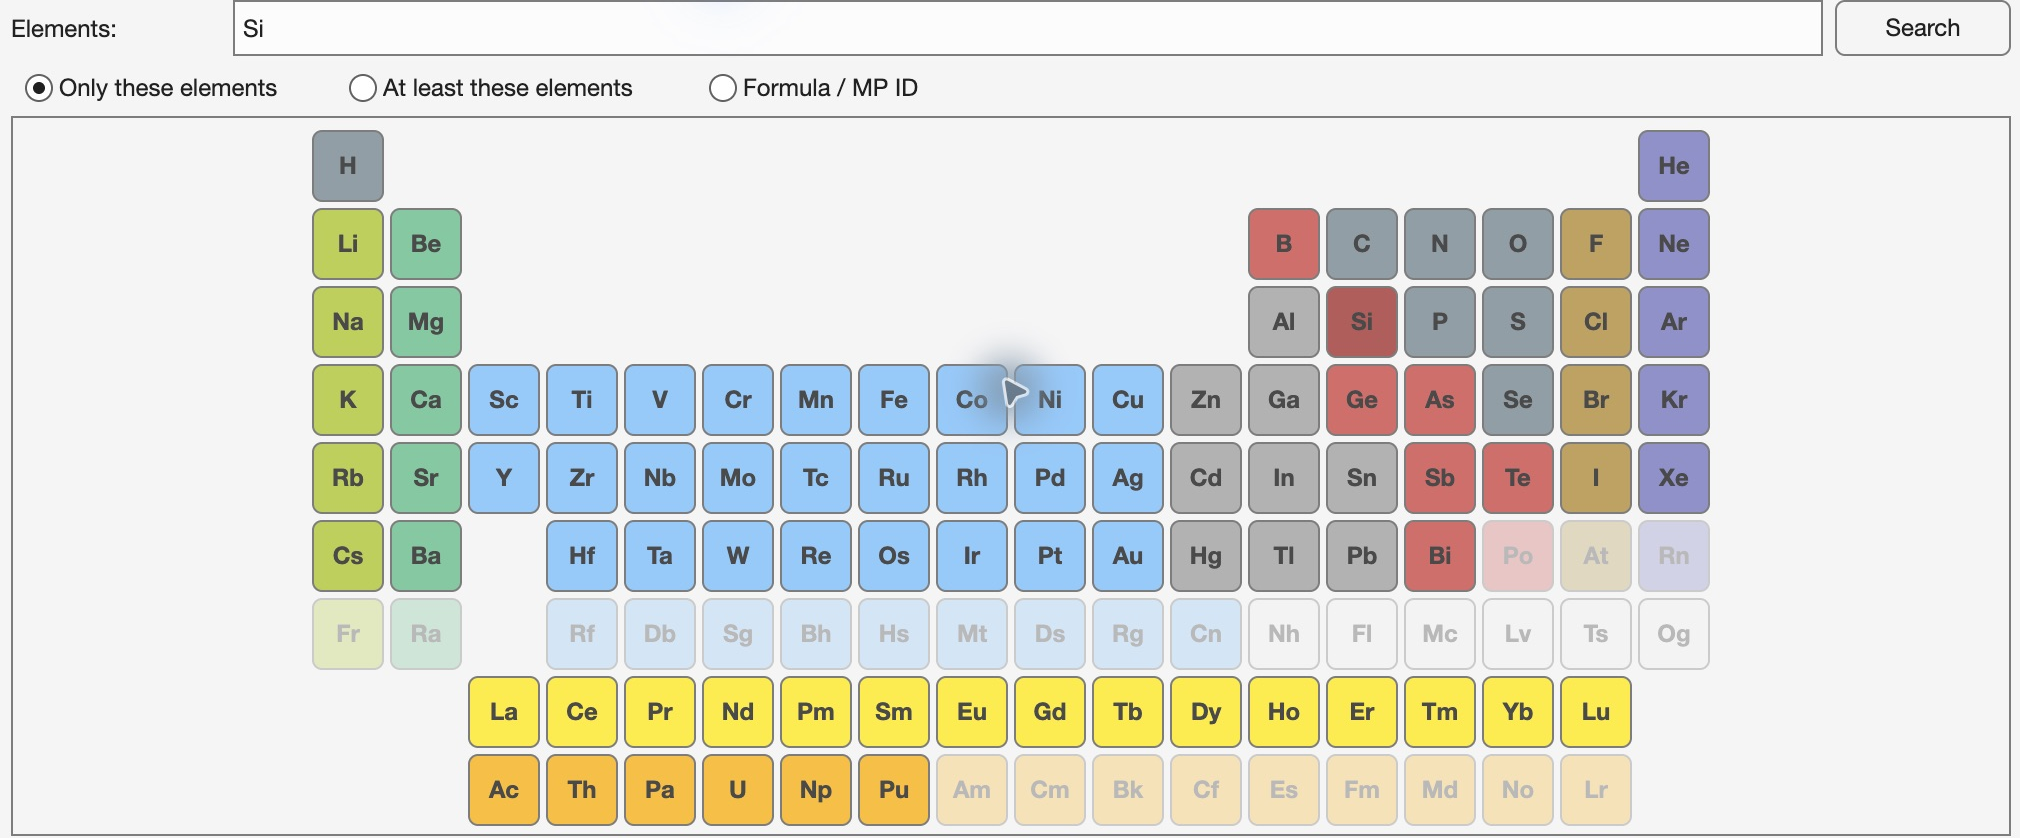
\includegraphics[width=\linewidth]{publication-assets/revision-materials-project-si-results.png}
\caption{Si selected in the periodic table with Only these elements to search elemental silicon. The search mode and elements appear above the results.}
\label{fig:mp-periodic-live}
\end{figure}

\begin{figure}[!htb]
\centering
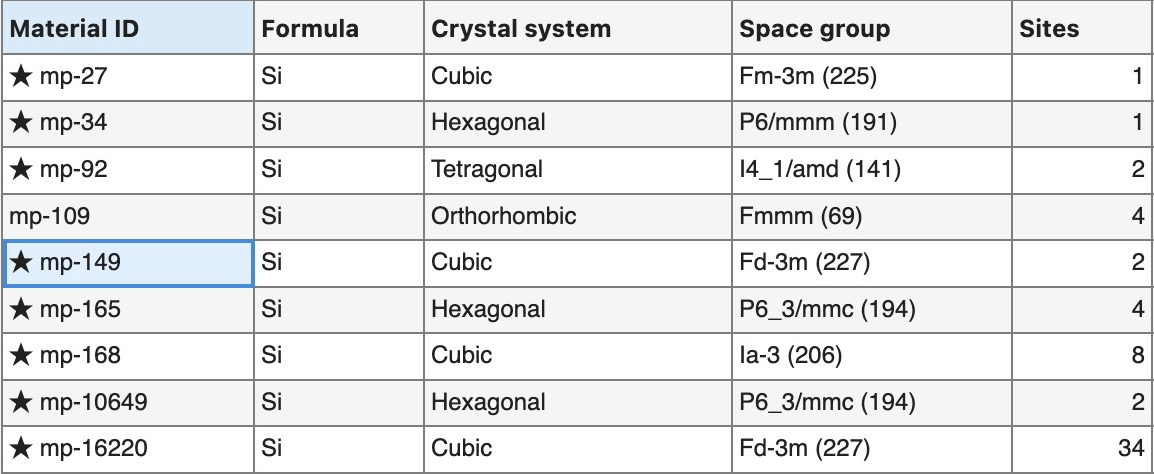
\includegraphics[width=\linewidth]{publication-assets/revision-materials-project-si-results-identity.png}
\caption{Identity columns in the silicon search results. The selected mp-149 record is Cubic, Fd-3m (227), with two atoms. Other silicon polymorphs are also listed.}
\label{fig:mp-results-live}
\end{figure}

\begin{figure}[!htb]
\centering
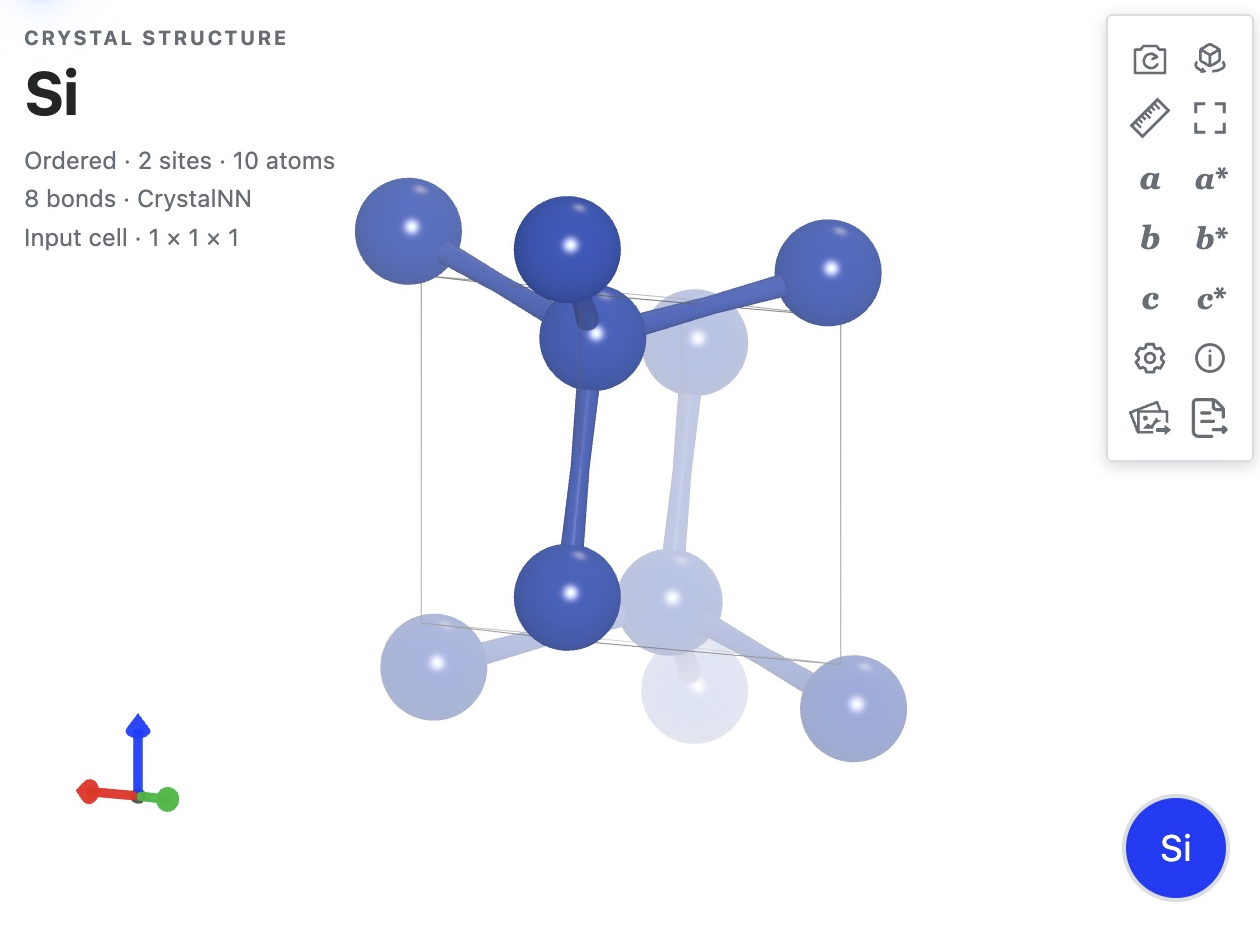
\includegraphics[width=\linewidth]{publication-assets/revision-materials-project-imported-si.png}
\caption{The silicon primitive-cell view opened after importing mp-149. The summary reports two independent sites; translucent images illustrate connections across periodic boundaries.}
\label{fig:mp-import-live}
\end{figure}

\section{Before you continue}
You should now be able to locate the imported silicon structure, open and close documents, expand and collapse side panels, and save a \file{.ks} project. Retain this silicon project and have the supplied hydrogen example ready before your first calculation. Later chapters return to silicon; use the structure file specified in each chapter when comparing numerical results.
